\chapter{Result and Discussion} % Main chapter title

\label{Chapter2.75} % Change X to a consecutive number; for referencing this chapter else where, use \ref{ChapterX}
%----------------------------------------------------------------------------------------
%	SECTION 1
%----------------------------------------------------------------------------------------

%-----------------------------------
%	SECTION 2
%-----------------------------------
\section{Before surface treatment}

Normalized cross-correlation evaluates the similarity between 2 patterns, the closer to 1, the higher the similarity. Here we compare the time-resolved PL spectra from every time tick with the first spectrum, the average value of this series of normalized cross-correlation reflects the general level of spectral stability of the measured point, additionally,the standard deviation of normalized cross-correlation indicates the speed of spectral changes.


\begin{figure}[h]
	\centering
	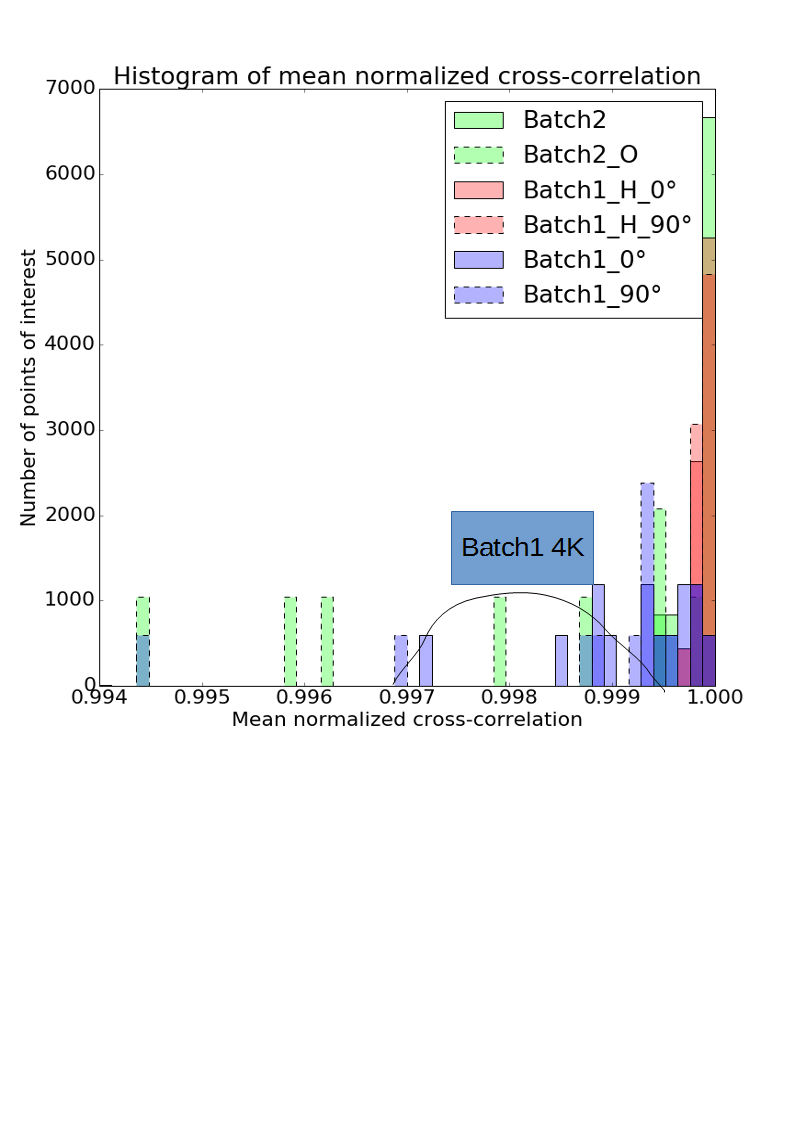
\includegraphics[width=1\linewidth]{Figures/pic/histall}
	\caption{Normalized histogram of mean normalized cross-correlation.}
	\label{fig:2015-09-07-ow-capture-20150907151210-744-1}
\end{figure}

Normalized cross-correlation evaluates the similarity between 2 patterns, the closer to 1, the higher the similarity. Here we compare the time-resolved PL spectra from every time tick with the first spectrum, the average value of this series of normalized cross-correlation reflects the general level of spectral stability of the measured point, additionally,the standard deviation of normalized cross-correlation indicates the speed of spectral changes.

As can be seen in Fig. 5.1, batch2 has better spectral stability than batch1. Larger diamond has better spectral stability fits the prediction that the spectral diffusion is related to the surface band bending. 

\section{power dependency}

\section{excitation polarisation}
\begin{figure}[h]
\centering
\includegraphics[width=0.7\linewidth]{"Figures/pic/excitation polarisation"}
\caption{Mean normalized cross-correlation against excitation polarisation. The error bar stand for standard deviation}
\label{fig:excitation-polarisation}
\end{figure}

 
It has been noticed that the mean cross correlation of nanodiamond batch1 at 4.7K is lower than it of the same batch of diamond at 20K. Such kind of behaviour has been reported on hydrogen terminated CVD nanodiamond, where the surface fermi level was unpinned, due to the low surface state density. When the surface state density is very low, we assume most of them are already occupied, so only very few electron exchange would exist between the bulk diamond and the surface states at reasonably low temperture. Taking fermi dirac distribution into consideration, to maintain a constant surface electron density, the value of $e^{\frac{E - E_{f}}}{kT}}$ need to be fixed, thus when the temperature increases, $E-E_{f}$ need to increase coorespondingly, which leads to the downwards movement of the relative position of surface trappig states regarding the band gap, resulting in the decrease of band bending near the surface as temperature raises. It has been reported that the denotated nanodiamond has similar surface states as hydrogen teminated bulk diamond, where due to the strong tendency for surface bond electrons to pair, a very low net surface unpaired electron density is expected, which is similar with the hydrogen terminated bulk diamond case.

\section{Oxidation}

\section{Hydrogen termination}


